\documentclass[15pt]{article}
\usepackage[utf8]{inputenc}
\usepackage[english, vietnamese]{babel}
\usepackage{fullpage}
\usepackage{tabto}

\title{geometry_computational}
\author{tu.nguyenanh.96 }
\date{November 2018}

\usepackage{natbib}
\usepackage{graphicx}

\begin{document}


\section{Giao Điểm Đoạn Thẳng Trong Mặt Phẳng}
\subsection{Ý Tưởng Thuật Toán}
Trong mục này, chúng ta sẽ đi giải quyết bài toán tìm giao điểm của các đoạn thẳng trong mặt phẳng được phát biểu cụ thể như sau: cho một tập $S$ gồm $n$ đoạn thẳng trên một mặt phẳng, liệt kê tất cả các giao điểm giữa các đoạn thẳng đó. \\

Để giải quyết được vấn đề này không khó, vì ta có thể đơn giản là kiêm tra qua tất cả các cặp cạnh trong mặt phẳng xem chúng nó giao nhau không. Giải thuật brute-force này chạy với độ phức tạp thời gian là $O(n^2)$. Tuy nhiên trong thực tế, hầu hết các cạnh không giao hoặc giao với một số ít các cạnh còn lại, vì thế số giao điểm có trên mặt phẳng nhỏ hơn nhiều so với bình phương số cạnh. Và vì vậy, ta mong muốn có một thuật toán chạy tốt hơn trong trường hợp này. Hay nói cách khác, một thuật toán mà tốc độ thời gian chạy không chỉ phụ thuộc vào số đoạn thẳng có trong mặt phẳng mà còn phụ thuộc số giao điểm giữa chúng. \\

Ta có nhận xét rằng, những cạnh ở gần nhau mới có thể giao nhau. Bây giờ, ta sẽ sự dủng quán sát này để xây dựng thuật toán toàn giao điểm. Gọi $S = \{s_1, s_2, ..., s_n \}$ là tập hợp các đoạn thẳng. Ta không muốn đi kiểm tra những đoạn thẳng nằm cách xa nhau trong mặt phẳng. Để làm được điều này, ta gọi $y-interval$ của một đoạn thẳng là hình chiếu của đoạn thẳng đó lên trục $Oy$. Ta có thể dễ dàng chứng minh rằng, nếu $y-interval$ của 2 đoạn thẳng không trùng nhau thì chúng sẽ không giao nhau. Vì thế ta chỉ cần phải đi kiểm tra sự giao nhau giữa 2 đoạn thẳng có $y-interval$ trùng lên nhau. \\

\begin{figure}[h!]
\centering
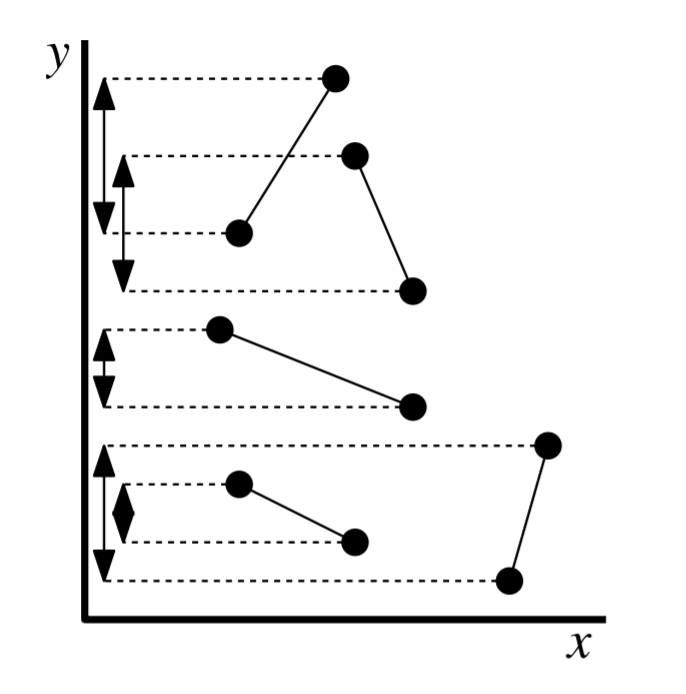
\includegraphics[scale=0.36]{./y_interval.png}
\caption{$y-interval$ các đoạn thẳng}
\label{fig:y-interval}
\end{figure}

Để làm được điều này ta sử dụng một đường thẳng quét (sweep line) $l$ đi từ trên xuống, xuất phát từ cạnh nằm trên cùng trong mặt phẳng. Khi đường thẳng quét từ trên xuống, ta chú ý đến tất các đoạn thẳng được giao với đường thẳng quét $l$ (ta còn gọi giải thuật này là sweep line algorithm). Ta gọi trạng thái của đường sweep line $l$ là tập hợp các đoạn thẳng giao với nó, trạng thái của đường thẳng quét sẽ được thay đổi trong quá trình $l$ được quét từ trên xuống. Trạng thái của đường thẳng quét chỉ cần phải cập nhật khi đường thẳng đi qua 1 số điểm đặc biệt. Ta gọi những điểm này là điểm sự kiện (event point). Trong giải thuật này, event points là các đầu mút của các đoạn thẳng. \\

Khi $l$ gặp 1 event point, nó phải cập nhập trạng thái (status) và thực hiện các kiểm tra giao điểm. Cụ thể là nếu event point là điểm đầu của đoạn thẳng, thì đoạn thẳng đó phải được thêm vào trong status, và sau đó đoạn thẳng được kiểm tra xem có giao điểm với các đoạn thẳng có trong status hay không. Nếu event point là điểm cuối của đoạn thẳng thì đoạn thẳng đước được bỏ ra khỏi status. \\

\begin{figure}[h!]
\centering
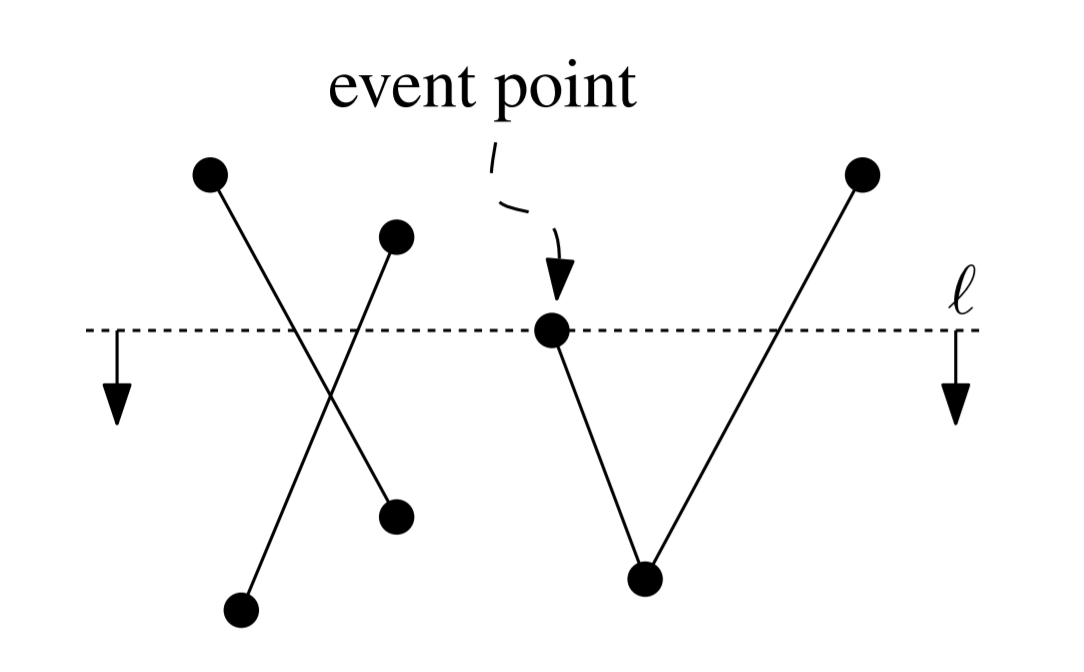
\includegraphics[scale=0.25]{./sweep_line.png}
\caption{Sweep line}
\label{fig:sweep_line}
\end{figure}

Tuy nhiên, nếu chỉ làm như vậy, vẫn có trường hợp ta vẫn phải kiểm tra một số bình phương số cạnh lần giao điểm giữa hai cạnh. Để khắc phục điều này ta sẽ sắp xếp các đoạn thẳng theo thứ tự trái qua phải, và ta chỉ kiểm tra giao điểm giữa 2 đoạn thẳng khí chụng nằm cạnh nhau. Khi sweep line $l$ tiếp tục đi xuống và vào một thời điểm nào đó thì thứ tự các cạnh trong status cần phải được thay đổi. Để giải quyết được vấn đề này, biến status phải được sắp xếp theo thứ tự từ trái sang phải. Và biến status không chỉ còn phải thay đổi khi gặp các đầu mút, mà biến status cũng phải được cập nhật thứ tự khi $l$ đi qua giao điểm (intersection point). \\

\textbf{Bồ đề 1.1} [1] Gọi $s_i$ và $s_j$ là hai đoan thẳng giao nhau tại một điểm trong $p$ và không có đoạn thẳng thứ ba cũng đi qua $p$. Khi đó tồn tại một điểm sự kiện nằm trên $p$ làm cho $s_i$ và $s_j$ kề nhau trong biến status.\\

Bồ đề trên bảo đảm tính đúng đắn của thuật toán ta vừa xây dựng: Khi sweep line gặp một event point, nó sẽ dừng lại để kiểm tra giao điểm hoặc đổi thứ tự các cạnh trong biến status. Các biến status gồm các đầu mút của các đoạn và giao điểm giữa chúng. Đầu mút của các đoạn ta hoàn toàn biết trước, còn các giao điểm ta phải tính toán trong quá trình sweep line $l$ quét mặt phẳng. \\

Các bước xử lý khi gặp event point được miêu tả cụ thể như sau. Khi đường thẳng quét gặp đinh trên của một đoạn thẳng, đoạn thẳng đó sẽ được kiểm tra giao điểm với 2 hàng xóm nằm cạnh nó trong biến status. Chỉ nhưng giao điểm nằm dưới đường thẳng $l$ mới cần được chú ý, vì những điểm nằm trên sweep line đã được xử lí xong. Khi đường thẳng quét gặp event point là giao điểm của 2 đoạn thẳng thì hai đoạn thẳng này đổi vị trí cho nhau trong event point, khi thay đổi vị trí, thuật toán tiếp tục kiểm tra giao điểm của 2 đoạn thẳng với cái hàng xóm mới. Tiếp theo, khi sweep line gặp event point là đầu mút dưới của một cạnh, ta xóa cạnh đó khỏi biến status. Khi đó 2 hàng xóm của cạnh được xóa trở thành hàng xóm của nhau và cần được kiểm tra xem chúng có giao điểm với nhau hay không. \\

\subsection{Cấu Trúc Dữ Liệu và Thuật Toán}
Đầu tiên ta cần xây dựng cấu trúc dữ liệu lưu các event point. Ở đây, ta sự dụng cấu trúc cây tự căn bằng để lưu các event point, và gọi cây này là $Q$. Ta cần thao tác xóa phần có tung độ lớn nhất trong cây event, trả về đỉnh đó và xử lí. Nếu hai event point có cùng tung độ thì ta sẽ lấy event có hoạnh độ thấp hơn. Cụ thể, ta thực hiện xây dựng cây event $Q$ như sau:  Ta định nghĩa phép so sánh $\prec$ giữa các event point. Với hai event point $p$ và $q$, ta có $p \prec q$ khi và chỉ khi $p_y > q_y$ hoặc $p_y = q_y$ và $p_x < q_x$. Các event point được luu trong cây $Q$ theo phép so sánh $\prec$. Với cấu trúc dữ liệu này, các thao tác thêm và xóa event đều mất $O(log m)$, trong đó $m$ là số các event đang được lưu ở trong cây $Q$. \\

Thứ hai, ta cần xây dựng cấu trúc dữ liệu cho biến biến status. Cấu trúc dữ liệu cho status, kí hiêu là $T$, được sử dụng để tìm kiếm hàng xóm của một đoạn thẳng $s$, thêm vào đó ta cũng cần phải thêm và xóa các đoạn. Ở đây, ta tiếp tục sử dụng cây tự cân bằng để giải quyết vấn đề này. Cụ thể như sau, ta lưu các đoạn giao với sweep line là các lá của cây tự cân bằng $T$ tho thứ tự từ trái sang phải. Tiếp theo, ta cần phải lưu thông tin các nút trong của cây để thuận tiện cho việc tìm kiếm. Tại mỗi đỉnh trong ta lưu cạnh nằm bên phải cùng của cây con trái đỉnh đó.

\begin{figure}[h!]
\centering
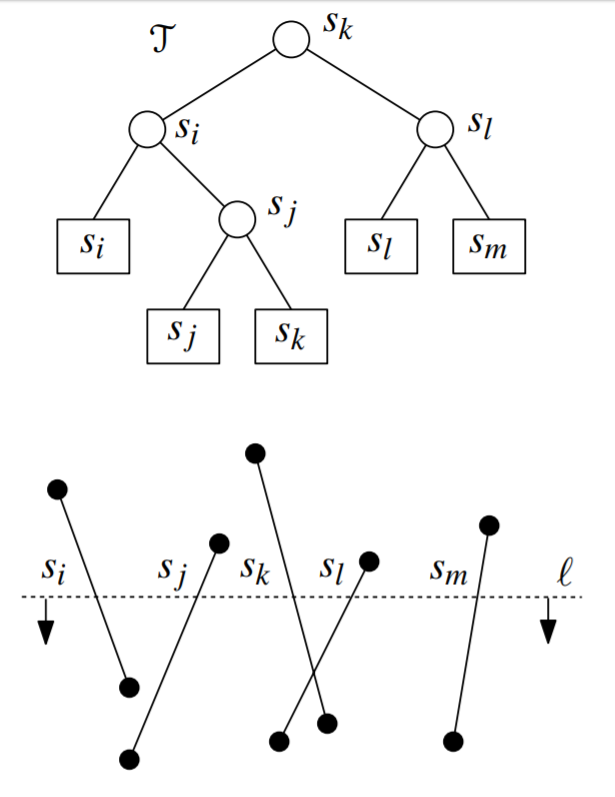
\includegraphics[scale=0.35]{./status_tree.png}
\caption{Ví dụ cây tự cân bằng status}
\label{fig:status tree exampels}
\end{figure}

Giả sử ta cần tìm trên $T$ cạnh nằm ngay bên trái của một điểm $p$ nằm trên đường thẳng quét. Tại mỗi đỉnh trong của cây, chúng ta kiểm tra xem $p$ nằm bên trái hay bên phải so với cạnh tương ứng với nút đó. Nếu cạnh đó nằm ở bên phải của điểm $p$, ta duyệt đến con trái của nút đó, và ngược lại đến khi ta duyệt đến một lá. Khi đó hoặc là nút ta thu được hoặc là lá nằm ngay bên trái so với nút đó tương ứng với đoạn thẳng mà ta cần tìm. Cuối cùng, ta có thể miêu tả thuật toán như sau. \\

\textbf{Giải Thuật} FindInterSections($S$) \\
\quad \textit{Đầu vào.} Tập hợp $S$ các đoạn thẳng trên mặt phẳng \\
\quad \textit{Đầu ra.} Tập hợp các giao điểm giữa các cạnh trong $S$
\begin{enumerate}
\item Khởi tạo cây event $Q$. Sau đó, lần lượt thêm các nút ứng với các đầu mút của các đoạn thẳng vào cây. Các đỉnh phía trên của các đoạn lưu thêm thông tin nó là đầu mút của cạnh nào.
\item Khởi tạo cây status $T$
\item \textbf{while} $Q$ khác rỗng
\item \quad \textbf{do} Xác định event point $p$ ơ trong $Q$ và xóa nó khổi cây
\item \quad \quad HandleEventPoint($p$)
\end{enumerate}

Trong phần trên, chúng ta đã miêu ta cách thuật toán xử lý khi gặp các event point. Trong trường hợp suy biến - các đoạn thẳng đồng quy - được xứ lý trong hàm HandleEventPoint($p$) như sau. \\

HandleEventPoint($p$)
\begin{enumerate}
\item Gọi $U(p)$ là tập hợp các đoạn thẳng có đầu mút trên là $p$ (Đối với đoạn thẳng nằm song song với đường thẳng quét, đầu mút bên trái được coi là đầu mút bên trên)
\item Tìm tất các đoạn thẳng trong cây status $T$ chưa $p$ (Các đoạn thẳng này liền kề nhau trên đường thẳng quét). Gọi $L(p)$ là tập hợp các đoạn thẳng có đầu mút dưới $p$ và $C(p)$ chứa các đoạn thẳng có điểm trong là $p$
\item \textbf{if} $U(p) \cup L(p) \cup C(p)$ chứa nhiều hơn 1 cạnh
\item \quad \textbf{then} Lưu $p$ là giao điểm
\item Xóa các cạnh $L(p) \cup C(p)$ khỏi $T$
\item Thêm các đoạn thẳng $U(p) \cup C(p)$ vào $T$. Thứ tự của các cạnh trên cây lúc này tuân theo thứ tự từ trái qua phải khi đường thẳng quét nằm ngay dưới $p$
\item \textbf{if} $U(p) \cup C(p) = \emptyset$
\item \quad \textbf{then} FindNewEvent($s_l, s_r, p$) trong đó $s_l$ và $s_r$ là cạnh nằm bên trái và bên phải của $p$
\item \textbf{else} Gọi $s'$ là đỉnh nằm tận cùng bên trái của tập $U(p) \cup C(p)$ trong cây $T$
\item \quad FindNewEvent($s_l, s', p$) trong đó $s_l$ là cạnh nằm bên trái $s'$
\item \quad Gọi $s''$ là cạnh nằm tận cùng bên phải $U(p) \cup C(p)$ trong cây $T$
\item \quad FindNewEVent($s'', s_r, p$) trong đó $s_r$ là cạnh nằm bên phải $s''$
\end{enumerate}

Thủ tục FindNewEvent($s_l, s_r, p$) được thực hiện như sau. \\

FindNewEvent($s_l, s_r, p$)
\begin{enumerate}
\item \textbf{if} $s_l$ và $_r$ cắt nhau tại một điểm nằm dưới đường thẳng quét hoặc thược đường quét và ở bên phải event point $p$, và giao điểm chưa xuất hiện trong cây event $Q$
\item \quad \textbf{then} Thêm giao điểm đó vào cây event $Q$
\end{enumerate}

\subsection{Tính Đúng Đắn và Độ Phức Tạp Thuật Toán}
Tính đúng đắn và độ phức tạp thuật toán được chứng minh trong [1] thông qua các bổ đề và định lý sau.\\

\textbf{Bổ đề 1.2} Thuật toán FindIntersections liệt kê ra được tất cả các giáo điểm giữa các đoạn thẳng. \\

\textbf{Bổ đề 1.3} Thuật toán FindIntersection chạy với độ phức tạp thời gian là $O(n log n + I log n$ trong đó $n$ là số cạnh trong mặt phẳng, và $I$ là sao giao điểm giữa các cạnh trong mặt phẳng. \\

\textbf{Định lý 1} Cho $S$ là tập hợp gồm $n$ đoạn thẳng trong mặt phẳng. Tất cả các giao điểm, cùng với các cạnh đi qua chúng đều có thể tìm kiếm trong thời gian $O(n log n + I log n)$ và chiếm $O(n)$ bộ nhớ, với $I$ là số giao điểm có trong mặt phẳng.


\section{Cấu Trúc Nửa Cạnh}
Chúng ta đã giải quyết được trường hợp đơn giản nhất của bài toán giao hai phân hoạch: giao của các đoạn thẳng trong mặt phẳng. Thực tế, các phân hoạch có cấu trúc phức tạp hơn: chúng là phân hoạch của một mặt phẳng thành các vùng được dán nhãn. Ví dụ: Một bản đồ chuyên về rừng ở Canada được phân cụm thành các vùng có nhãn "thông", "rụng lá", "bạch dương", "hỗn hợp".\\

Trước khi đưa ra giải thuật về việc tính toán giao của hai phân hoạch, ta phải xây dựng một biểu diễn phù hợp cho các phân hoạch. Lưu một phân hoạch như một tập hợp các đoạn thẳng không phải là một ý tưởng hay. Việc liệt kê biên của một vùng sẽ khá phức tạp. Nó sẽ tốt hơn nếu ta kết hợp các thông tin cấu trúc như: các đoạn thẳng nào là biên của vùng, vùng nào liền kề, v.v...\\

Trong bản báo cáo này, ta chỉ xét các phân hoạch phẳng được tạo ra bởi các đồ thị phẳng. Phân hoạch như vậy được gọi là liên thông nếu đồ thị tạo ra nó liên thông. Tương ứng mỗi nút của đồ thị là một đỉnh, mỗi cung được gọi là một cạnh. Ta chỉ xét các cạnh là đoạn thẳng, mặc dù về nguyên tắc các cạnh không cần phải thẳng. Một mặt của phân hoạch là một tập con lớn nhất (theo nghĩa bao hàm) của đồ thị và không bao gồm các đỉnh. Thế nên mặt là một miền đa giác mở mà biên của nó được giới hạn bởi các cạnh và các đỉnh của phân hoạch. Độ phức tạp của phân hoạch là tổng số đỉnh, số cạnh và số mặt của phân hoạch đó. Nếu một đỉnh là đầu mút của cạnh thì ta nói đỉnh và cạnh đó kề nhau. Tương tự, mặt và cạnh thuộc biên của nó kề nhau, mặt và đỉnh thuộc biên của nó kề nhau. \\

Một cấu trúc nửa cạnh lữu trữ các thông tin về mặt, cạnh và đỉnh của phân hoạch. Bên cạnh thông tin hình học, ta có thể lưu trữ thêm các thông tin bổ sung. Để quét biên của một mặt phẳng theo thứ tự ngược chiều kim đồng hồ, ta chỉ cần lưu lại con trỏ mỗi cạnh tới cạnh tiếp theo. Đôi khi, ta cũng cần thiết phải đi theo đường biên theo hướng ngược lại, nên ta lưu lại con trỏ tới cạnh liền trước. Một cạnh thuộc hai mặt nên ta cũng cần hai con trỏ để lưu trữ nó. Nó rất thuận tiện để xét hai mặt khác nhau của một cạnh như là hai nửa cạnh. Điều đó có nghĩa từ nửa cạnh ta có thể biết được 1 mặt chứa nửa cạnh đó. Hai nửa cạnh của một cạnh ta gọi chúng là hai nửa cạnh đối nhau hay hai nửa cạnh song sinh. Để xác định hướng một nửa cạnh: theo ngược chiều kim đồng hồ, ta đi xung quanh biên của mặt của nửa cạnh sao cho tay trái ta hướng vào miền trong của mặt. Sau khi xác định hướng của một nửa cạnh, ta dễ dàng xác định điểm đầu và điểm cuối của nửa cạnh. Nếu nửa cạnh $\vec{e}$ có điểm đầu là $v$ và điểm cuối là $w$ thì nửa cạnh đối của $\vec{e}$ sẽ có điểm đầu là $w$ và điểm cuối là $v$. Để biết biên của một mặt, ta cần lưu lại con trỏ trong thuộc tính mặt một nửa cạnh bất kỳ thuộc mặt đó. Xuất phát từ nửa cạnh đó ta có thể di chuyển tới nửa cạnh tiếp theo và quét hết biên của mặt chứa nửa cạnh đó. \\

\begin{figure}[h!]
\centering
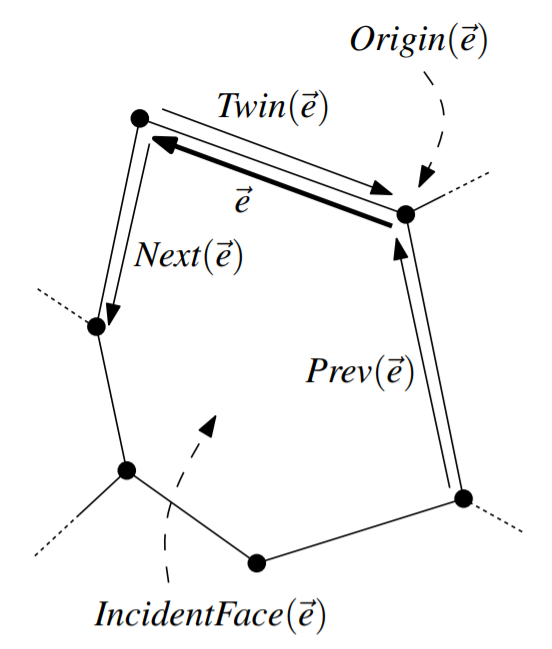
\includegraphics[scale=0.38]{./dcel1.png}
\caption{Cấu trúc nửa cạnh}
\label{fig: cấu trức nửa cạnh}
\end{figure}

Tóm lại, Cấu trúc nửa cạnh bao gồm 3 thuộc tính: các đỉnh, các mặt, các nửa cạnh. Trong đó:
\begin{itemize}
    \item Các đỉnh $v$ lưu lại tọa độ của $v$ trong một trường gọi là $Coordinates$ và con trỏ $IncidentEdge()$ của một nửa cạnh có $v$ làm gốc.
    \item Các mặt $f$ lưu con trỏ $OuterComponent$ cho một  nửa cạnh thuộc biên của $f$. Đối với mặt ngoài (mặt không giới hạn), con trỏ này là \textbf{nil}. Các mặt cũng lưu danh sách $InnerComponent$ - chứa các con trỏ chỉ tới một nửa cạnh tương ứng với mỗi hố trong mặt đó.
    \item Các nửa cạnh $\vec{e}$ lưu con trỏ $Origin$ - gốc của nửa cạnh, con trỏ $Twin$ - nửa cạnh đối của $\vec{e}$ và con trỏ $IncidentFace$ - mặt kề với nửa cạnh $\vec{e}$. Chúng ta không cần lưu đỉnh cuối của $\vec{e}$ vì nó là $Origin(Twin(\vec{e}))$. Gốc của nửa cạnh được chọn sao cho $IncidentFace(\vec{e})$ nằm ở bên trái của $\vec{e}$ khi ta đi từ đỉnh gốc đến đỉnh cuối của $\vec{e}$. Bản ghi nửa cạnh cũng lưu con trỏ $Next(\vec{e})$ và $Prev(\vec{e})$ tương ứng với cạnh tiếp theo và cạnh trước thuộc biên của $IncidentFace(\vec{e})$. Như vậy, $Next(\vec{e})$ là nửa cạnh thuộc biên của  $IncidentFace(\vec{e})$ mà có đỉnh cuối của $\vec{e}$ là gốc và $Prev(\vec{e})$ là nửa cạnh thuộc biên của $IncidentFace(\vec{e})$ mà có $Origin(\vec{e})$ là đỉnh cuối.
\end{itemize}

\begin{figure}[h!]
\centering
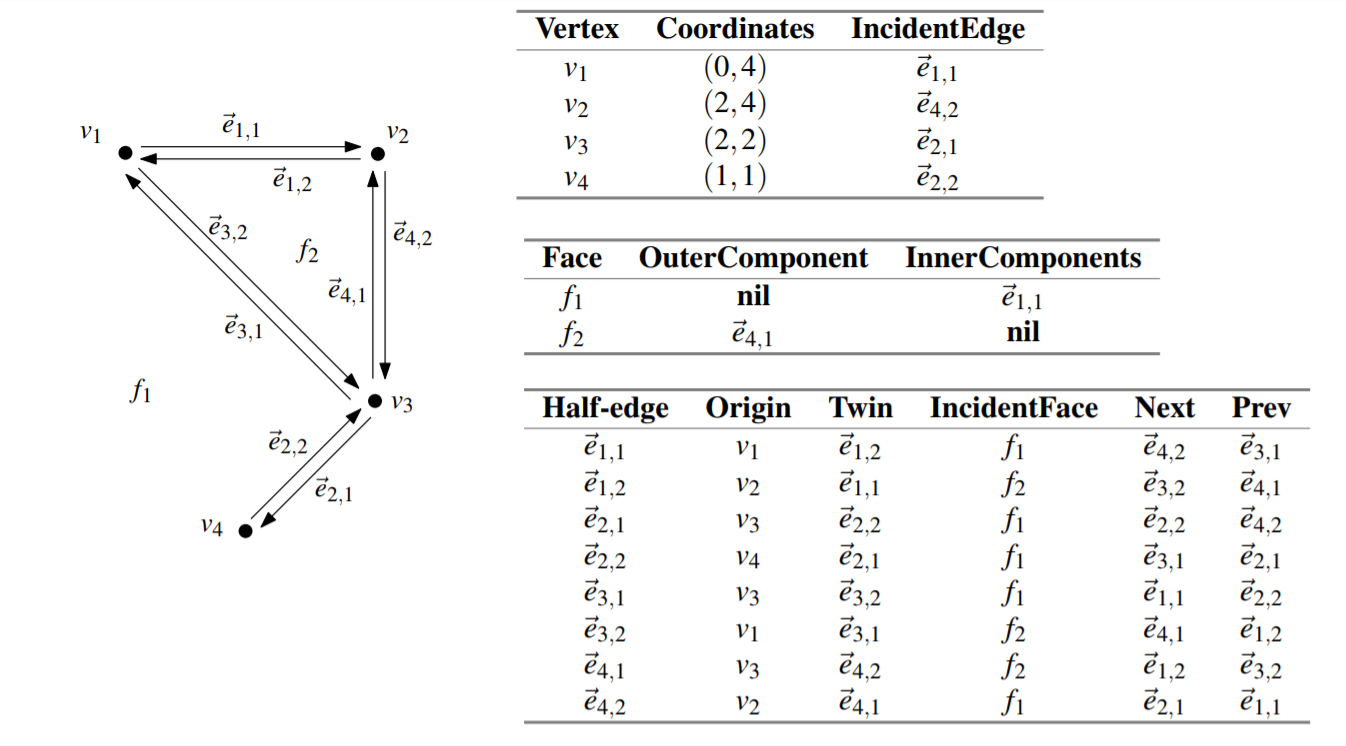
\includegraphics[scale=0.5]{./dcel2.png}
\caption{Ví dụ về cấu trúc nửa cạnh}
\label{fig: ví dụ về cấu trúc nửa cạnh}
\end{figure}

\section{Giao Phân Hoạch}
\subsection{Phát Biểu Bài Toán}
Bây giờ, ta đã có cấu trúc dữ liệu nửa cạnh là một phương pháp tốt để biểu diện một phân hoạch. Bài toán đặt ra ở đây là nếu có hai phân hoạch được đặt chồng lên nhau thì khi đó các mặt mới được tạo ra và việc cập nhật lại thông tin ở trên dữ liệu nửa cạnh sẽ như thế nào. \\

Cụ thể, ta kí hiệu giao của phần hoạch $S_1$ và phân hoạch $S_2$ là phân hoạch $O(S_1, S_2)$ và $f$ được gọi là một mặt trong phân hoạch mới nếu tồn tại $f_1$ thuộc $S_1$ và $f_2$thuộc $S_2$ sao cho $f$ là tập con liên thông cực đại (theo nghĩa bao hàm) của $f_1 \cap f_2$. Mô tả như hình vẽ.\\

\begin{figure}[h!]
\centering
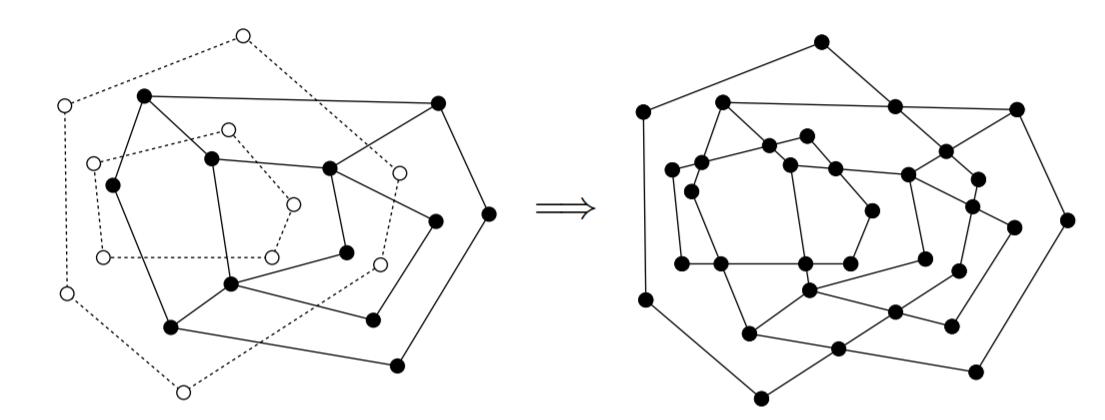
\includegraphics[scale=0.5]{./mapoverlay_example.png}
\caption{Giao hai phân hoạch}
\label{fig: giao hai phân hoạch}
\end{figure}

Bài toán đặt ra ở đây là chúng ta cần phải xây dựng lại cấu trúc nửa cạnh cho phân hoạch mới được tạo ra từ hai phân hoạch.

\subsection{Xây Dựng Thuật Toán}
Chúng ta thấy rằng các cạnh của phân hoạch $S_1$ giao cắt với các cạnh của phân hoạch $S_2$ tạo thêm các đỉnh, canh và mặt mới. Tuy nhiên ta không cần phải cập nhật thông tin của tất cả các cạnh mà chỉ cần quan tâm đến giao điểm giữa cạnh của phân hoạch này với cạnh của phân hoạch kia. Và các thông tin về mặt của phân hoạch mới hoàn toàn có thể xây dựng thông qua dữ liệu về các nửa cạnh mới. \\

Như vậy việc đầu tiên ta cần làm là tìm giao điểm của các cạnh giữa hai phân hoạch, cập nhập thêm các đỉnh và nửa cạnh mới. Để làm được điều này, ta tận dụng giải thuật tìm giao điểm giữa các cạnh mà ta đã biết. Đầu tiên, ta ghép danh sách nửa cạnh $D_1$ của phân hoạch $S_1$ và danh sách nửa cạnh $D_2$ của phân hoạch $S_2$ thành danh sách nửa cạnh mới $D$. Sau đó chạy giải thuật tìm giao điểm trên danh sách nửa cạnh $D$. Ở đây, có khác so với thuật toán giao cắt các đoạn thẳng miêu tả ở phần trước đó là trong quá trình quét mặt phẳng, ta sẽ đồng thời xây dựng cấu trúc nửa cảnh. \\

Trước tiên, ta miêu tả giải thuật quét mặt phẳng để xây dựng nên các nửa cạnh, còn thông tin về mặt ta sẽ xử lý sau. Ta chạy giải thuật quét mặt phẳng tìm giao điểm như đã miêu tả ở phần trên cho tập cạnh $D$. Ngoài việc, xử lý hai cấu trúc cây event và cây status $Q$ và $T$, bây giờ ta lưu thêm danh sách của nửa cạnh $D$. Khi khởi tạo, danh sách này gồm bản sao danh sách nửa cạnh của hai phân hoạch $S_1$ và $S_2$. Trong quá trình quét mặt phẳng, ta sẽ dần dần cập nhập danh sách nửa cạnh trở thành danh sách nửa cạnh đúng. \\

Khi đường thẳng quét gặp một event point, đầu tiên, ta sẽ cập nhập cây event $Q$ và cây status $T$. Nếu điểm sự kiện đó chỉ kề với những cạnh thuộc cùng một phân hoạch, thì khi đó, đỉnh này là đỉnh có thể sự dụng lại được và ta không cần phải làm gì thêm. Nếu đỉnh kề với các cạnh thuộc cả hai phân hoạch, khi đó ta phải cập nhập thông tin cho $D$. Để làm được điều này, ta đi xét 3 trường hợp sau. \\

\begin{figure}[h!]
\centering
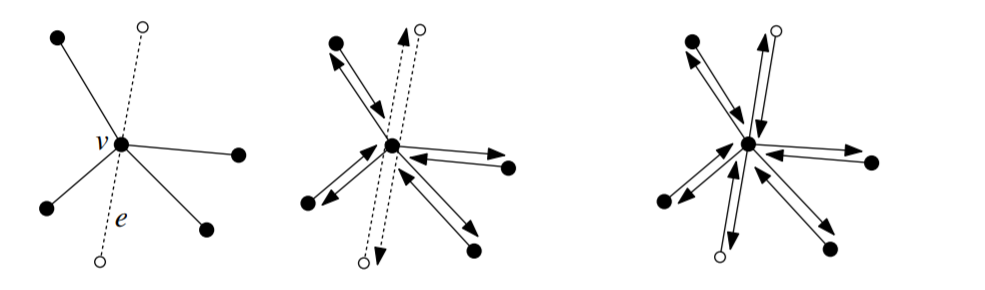
\includegraphics[scale=0.5]{./vertex_from_subdivisions.png}
\caption{Xác định con trỏ next, prev}
\label{fig: giao hai phân hoạch}
\end{figure}

Trường hợp thứ nhất là trong quá trình quét ta thấy cạnh $e$ của $S_1$ đi qua đỉnh $v$ của $S_2$. Cạnh $e$ khi đó cần phải được thay thế bằng hai cạnh $e'$ và $e''$. Trong dánh sách nửa cạnh $D$, hai cạnh mới thêm này tương ứng với 4 nửa cạnh. Đầu tiên, ta tạo mới 2 nửa cạnh đều có gốc là $v$, hai nửa cạnh ứng với cạnh $e$ được giữ nguyên gốc là hai đầu mút của cạnh $e$. sau đó, ta gán 2 nửa cạnh này là twin với 2 nửa cạnh mới được tạo. Khi đó $e'$ và $e''$ được biểu diện 2 nửa cạnh, một mới được tạo, một được lấy từ nửa cạnh của $e$. Bây giờ, ta chỉ cần tìm các con trỏ next và prev cho 4 nửa cạnh này. Ta xử lý các trường hợp dính tới 2 đầu mút của cạnh $e$ được miêu tả như hình vẽ. \\

Đối với các trường hợp liên quan tới đỉnh $v$, ta cần phải gán các con trỏ next và prev cho 4 nửa cạnh biểu diễn cho $e'$ và $e''$

\subsection{Tính Đúng Đắn và Độ Phức Tạp}
\section{Kết Quả}
\section{Conclusion}
``I always thought something was fundamentally wrong with the universe'' \citep{adams1995hitchhiker}

\bibliographystyle{plain}
\bibliography{references}
\end{document}